\documentclass[12pt,a4paper]{article}

% ─── Page Layout ───────────────────────────────────────────────────────────────
\usepackage[a4paper, margin=0.8in, headheight=14pt]{geometry}

% ─── Fonts (XeLaTeX) ───────────────────────────────────────────────────────────
\usepackage{fontspec}
\usepackage{unicode-math}
\setmainfont{TeX Gyre Pagella}
\setmonofont[Scale=0.88]{TeX Gyre Cursor}
\setmathfont{Latin Modern Math}

% ─── Packages ──────────────────────────────────────────────────────────────────
\usepackage{xcolor}
\usepackage{colortbl}
\usepackage{titlesec}
\usepackage{enumitem}
\usepackage{tabularx}
\usepackage{booktabs}
\usepackage{array}
\usepackage{amsmath}
\usepackage{tikz}
\usetikzlibrary{shapes.geometric, arrows.meta, positioning, calc, fit, decorations.pathreplacing, patterns}
\usepackage[american]{circuitikz}
\usepackage{tcolorbox}
\tcbuselibrary{skins, breakable}
\usepackage{hyperref}
\usepackage{fancyhdr}
\usepackage{graphicx}
\usepackage{microtype}
\hyphenpenalty=10000
\exhyphenpenalty=10000
\sloppy
\usepackage{caption}
\usepackage{setspace}
\usepackage{multirow}
\usepackage{tocloft}

% ─── Q&A helper ────────────────────────────────────────────────────────────────
\newcommand{\Q}[1]{\textbf{#1}\par\noindent\ignorespaces}

% ─── Colour Palette ────────────────────────────────────────────────────────────
\definecolor{myred}{RGB}{196,30,58}
\definecolor{mydark}{RGB}{30,30,50}
\definecolor{mygreen}{RGB}{14,120,80}
\definecolor{myteal}{RGB}{0,130,140}
\definecolor{myamber}{RGB}{180,100,0}
\definecolor{mypurple}{RGB}{100,30,160}
\definecolor{mygray}{RGB}{246,247,249}
\definecolor{mgframe}{RGB}{180,185,200}
\definecolor{watermark}{RGB}{145,150,170}
\definecolor{hdrred}{RGB}{250,232,235}
\definecolor{hdrgreen}{RGB}{220,244,233}
\definecolor{hdrteal}{RGB}{220,242,244}
\definecolor{hdramber}{RGB}{253,242,215}
\definecolor{hdrpurple}{RGB}{238,228,255}
\definecolor{hdrgray}{RGB}{238,240,245}
\definecolor{rowalt}{RGB}{250,251,253}

% ─── Section Formatting ────────────────────────────────────────────────────────
\titleformat{\section}{\large\bfseries\color{myred}}{\thesection.}{0.5em}{}[\vspace{1pt}{\color{myred}\rule{\linewidth}{0.8pt}}]
\titleformat{\subsection}{\normalsize\bfseries\color{myteal}}{\thesubsection}{0.5em}{}
\titlespacing*{\section}{0pt}{18pt}{7pt}
\titlespacing*{\subsection}{0pt}{11pt}{4pt}

% ─── Paragraph ─────────────────────────────────────────────────────────────────
\setlength{\parindent}{0pt}
\setlength{\parskip}{4pt}

% ─── TOC Styling ───────────────────────────────────────────────────────────────
\renewcommand{\cfttoctitlefont}{\large\bfseries\color{myred}}
\renewcommand{\cftaftertoctitle}{\par\noindent{\color{myred}\rule{\linewidth}{0.8pt}}}
\setlength{\cftbeforetoctitleskip}{0pt}
\setlength{\cftaftertoctitleskip}{6pt}
\renewcommand{\cftsecfont}{\normalsize\bfseries\color{mydark}}
\renewcommand{\cftsecpagefont}{\normalsize\bfseries\color{mydark}}
\renewcommand{\cftsecleader}{\cftdotfill{\cftdotsep}}
\setlength{\cftbeforesecskip}{7pt}
\renewcommand{\cftsubsecfont}{\small\color{mydark}}
\renewcommand{\cftsubsecpagefont}{\small\color{mydark}}
\setlength{\cftbeforesubsecskip}{3pt}
\setlength{\cftsubsecindent}{1.4em}

% ─── Table helpers ─────────────────────────────────────────────────────────────
\renewcommand{\arraystretch}{1.45}
\setlength{\tabcolsep}{6pt}
\arrayrulecolor{mydark}
\newcolumntype{B}[1]{>{\small\bfseries\raggedright\arraybackslash}m{#1}}
\newcolumntype{Y}{>{\small\raggedright\arraybackslash}X}
\renewcommand{\tabularxcolumn}[1]{m{#1}}

% ─── Header / Footer ───────────────────────────────────────────────────────────
\pagestyle{fancy}
\fancyhf{}
\fancyhead[L]{\small\color{myred}\textbf{PE-EC802C}\;\color{mydark}--- VLSI Design Automation}
\fancyhead[R]{\small\color{myteal}\textbf{Module 1 Notes}}
\fancyfoot[C]{\small\color{mydark}\thepage}
\fancyfoot[R]{\small\color{watermark}\textit{\copyright\ Biraj Sarkar}}
\renewcommand{\headrulewidth}{0.5pt}
\renewcommand{\footrulewidth}{0.3pt}

% ─── Hyperref ──────────────────────────────────────────────────────────────────
\hypersetup{colorlinks=true, linkcolor=myteal, urlcolor=myteal,
  pdfauthor={Biraj Sarkar}, pdftitle={PE-EC802C --- Module 1 Notes}}

% ─── tcolorbox styles ──────────────────────────────────────────────────────────
\tcbset{
  tikzbox/.style={colback=mygray, colframe=mgframe, boxrule=0.6pt, arc=4pt,
    left=8pt, right=8pt, top=6pt, bottom=6pt,
    colbacktitle=mgframe, coltitle=mydark, fonttitle=\small\bfseries},
  defbox/.style={colback=hdrgreen, colframe=mygreen, boxrule=0.8pt, arc=4pt,
    left=9pt, right=9pt, top=6pt, bottom=6pt,
    colbacktitle=mygreen, coltitle=white, fonttitle=\small\bfseries},
  formulabox/.style={colback=hdrteal, colframe=myteal, boxrule=0.8pt, arc=4pt,
    left=9pt, right=9pt, top=7pt, bottom=7pt,
    colbacktitle=myteal, coltitle=white, fonttitle=\small\bfseries},
  examplebox/.style={colback=hdramber, colframe=myamber, boxrule=0.8pt, arc=4pt,
    left=9pt, right=9pt, top=6pt, bottom=6pt,
    colbacktitle=myamber, coltitle=white, fonttitle=\small\bfseries},
  masonbox/.style={colback=hdrpurple, colframe=mypurple, boxrule=0.8pt, arc=4pt,
    left=9pt, right=9pt, top=6pt, bottom=6pt,
    colbacktitle=mypurple, coltitle=white, fonttitle=\small\bfseries},
  exambox/.style={colback=hdrpurple, colframe=mypurple, boxrule=1pt, arc=5pt,
    left=10pt, right=10pt, top=8pt, bottom=8pt,
    colbacktitle=mypurple, coltitle=white, fonttitle=\bfseries,
    breakable, title after break={\textbf{Frequently Asked / Viva Questions (contd.)}}}
}
\tcbset{breakable}

% ─── TikZ styles ───────────────────────────────────────────────────────────────
\tikzset{
  block/.style={rectangle, draw=myteal, fill=hdrteal,
    text width=2.4cm, align=center, minimum height=0.95cm,
    font=\small, rounded corners=3pt, line width=0.7pt},
  redblock/.style={rectangle, draw=myred, fill=hdrred,
    text width=2.4cm, align=center, minimum height=0.95cm,
    font=\small, rounded corners=3pt, line width=0.7pt},
  sumjunc/.style={circle, draw=myamber, fill=hdramber,
    minimum size=0.62cm, font=\small, line width=0.8pt},
  arrow/.style={-Stealth, thick, color=mydark},
  line/.style={thick, color=mydark}
}

% ═══════════════════════════════════════════════════════════════════════════════
\begin{document}
% ═══════════════════════════════════════════════════════════════════════════════

\begin{center}
  {\LARGE\bfseries\color{myred} PE-EC802C --- VLSI Design Automation}\\[5pt]
  {\normalsize\color{mydark} Semester VIII \quad$\bullet$\quad 3L:0T:0P \quad$\bullet$\quad 3 Credits}\\[3pt]
  {\normalsize\color{myteal}\textbf{Module 1: Introduction to VLSI Design Methodologies \& Algorithms}}\\[3pt]
  {\small\color{mydark} CGEC \;$|$\; B.Tech ECE (2023--27) \;$|$\; \textit{Biraj Sarkar}}
\end{center}
\vspace{2pt}
\noindent{\color{myred}\rule{\linewidth}{1.5pt}}
\vspace{2pt}

\hypersetup{linkcolor=mydark}
\tableofcontents
\hypersetup{linkcolor=myteal}
\newpage

% ===============================================================================
\section{VLSI Design Flow \& Abstraction Levels}
% ===============================================================================

\begin{tcolorbox}[defbox, title={VLSI Design Automation}]
  \textbf{VLSI Design Automation} refers to the use of computer-aided design (CAD) software tools to automate the translation of a high-level description of an electronic system into a physical layout fabricated on a silicon wafer. It covers synthesis, optimization, physical layout, verification, and testing.
\end{tcolorbox}

\subsection{Gajski-Kuhn Y-Chart}
The Gajski-Kuhn Y-Chart is a framework that describes electronic system design using three distinct domains represented as three axes of a Y:
\begin{itemize}[leftmargin=*, itemsep=2pt]
  \item \textbf{Behavioral Domain:} Describes \textit{what} the system does in terms of function, transfer functions, executable algorithms, and state machines.
  \item \textbf{Structural Domain:} Describes \textit{how} the system is connected in terms of hardware entities like registers, ALUs, logic gates, and transistors.
  \item \textbf{Physical Domain:} Describes the physical implementation details on silicon, including floorplans, cell placement, macro routing, and transistor layouts.
\end{itemize}

The concentric rings crossing the three axes represent the \textbf{levels of abstraction}: System, Register Transfer Level (RTL), Gate/Logic, and Circuit/Transistor levels.

\begin{tcolorbox}[tikzbox, title={Gajski-Kuhn Y-Chart}]
\centering
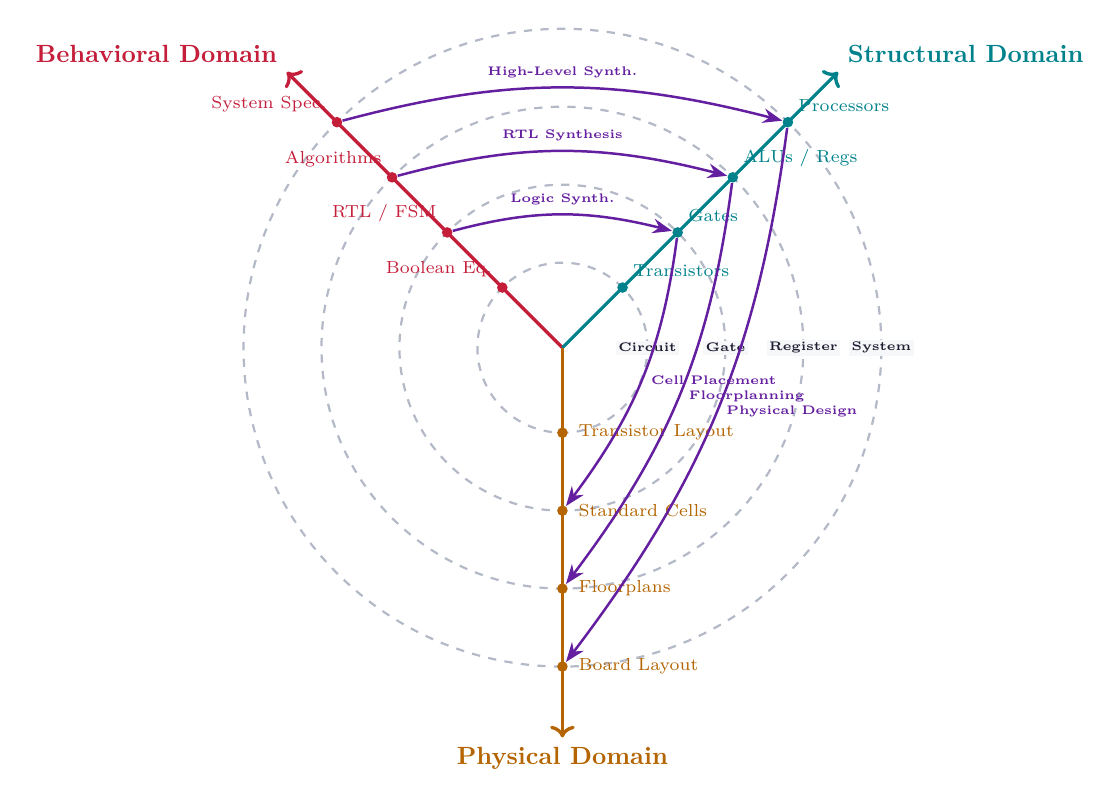
\begin{tikzpicture}[scale=0.9, transform shape]
  % Draw axes
  \draw[line, ->, line width=1.2pt, color=myred] (0,0) -- (135:5.5) node[above left, font=\bfseries] {Behavioral Domain};
  \draw[line, ->, line width=1.2pt, color=myteal] (0,0) -- (45:5.5) node[above right, font=\bfseries] {Structural Domain};
  \draw[line, ->, line width=1.2pt, color=myamber] (0,0) -- (270:5.5) node[below, font=\bfseries] {Physical Domain};
  
  % Concentric circles (dashed, gray) representing abstraction levels
  \foreach \r/\name in {1.2/Circuit, 2.3/Gate, 3.4/Register, 4.5/System} {
    \draw[dashed, color=mgframe, line width=0.8pt] (0,0) circle (\r);
    \node[color=mydark, font=\tiny\bfseries, fill=mygray, inner sep=1pt] at (0:\r) {\name};
  }

  % Dots on Behavioral Axis (135 degrees)
  \node[circle, fill=myred, inner sep=1.5pt] (b1) at (135:1.2) {};
  \node[above left=1pt, font=\scriptsize, color=myred] at (135:1.2) {Boolean Eq.};
  \node[circle, fill=myred, inner sep=1.5pt] (b2) at (135:2.3) {};
  \node[above left=1pt, font=\scriptsize, color=myred] at (135:2.3) {RTL / FSM};
  \node[circle, fill=myred, inner sep=1.5pt] (b3) at (135:3.4) {};
  \node[above left=1pt, font=\scriptsize, color=myred] at (135:3.4) {Algorithms};
  \node[circle, fill=myred, inner sep=1.5pt] (b4) at (135:4.5) {};
  \node[above left=1pt, font=\scriptsize, color=myred] at (135:4.5) {System Spec.};

  % Dots on Structural Axis (45 degrees)
  \node[circle, fill=myteal, inner sep=1.5pt] (s1) at (45:1.2) {};
  \node[above right=1pt, font=\scriptsize, color=myteal] at (45:1.2) {Transistors};
  \node[circle, fill=myteal, inner sep=1.5pt] (s2) at (45:2.3) {};
  \node[above right=1pt, font=\scriptsize, color=myteal] at (45:2.3) {Gates};
  \node[circle, fill=myteal, inner sep=1.5pt] (s3) at (45:3.4) {};
  \node[above right=1pt, font=\scriptsize, color=myteal] at (45:3.4) {ALUs / Regs};
  \node[circle, fill=myteal, inner sep=1.5pt] (s4) at (45:4.5) {};
  \node[above right=1pt, font=\scriptsize, color=myteal] at (45:4.5) {Processors};

  % Dots on Physical Axis (270 degrees)
  \node[circle, fill=myamber, inner sep=1.5pt] (p1) at (270:1.2) {};
  \node[right=3pt, font=\scriptsize, color=myamber] at (270:1.2) {Transistor Layout};
  \node[circle, fill=myamber, inner sep=1.5pt] (p2) at (270:2.3) {};
  \node[right=3pt, font=\scriptsize, color=myamber] at (270:2.3) {Standard Cells};
  \node[circle, fill=myamber, inner sep=1.5pt] (p3) at (270:3.4) {};
  \node[right=3pt, font=\scriptsize, color=myamber] at (270:3.4) {Floorplans};
  \node[circle, fill=myamber, inner sep=1.5pt] (p4) at (270:4.5) {};
  \node[right=3pt, font=\scriptsize, color=myamber] at (270:4.5) {Board Layout};

  % Translation arrows (curved synthesis/implementation steps)
  \draw[arrow, bend left=15, color=mypurple, line width=0.9pt] (b4) to node[midway, above, font=\tiny\bfseries] {High-Level Synth.} (s4);
  \draw[arrow, bend left=15, color=mypurple, line width=0.9pt] (s4) to node[midway, right, font=\tiny\bfseries] {Physical Design} (p4);
  
  \draw[arrow, bend left=15, color=mypurple, line width=0.9pt] (b3) to node[midway, above, font=\tiny\bfseries] {RTL Synthesis} (s3);
  \draw[arrow, bend left=15, color=mypurple, line width=0.9pt] (s3) to node[midway, right, font=\tiny\bfseries] {Floorplanning} (p3);

  \draw[arrow, bend left=15, color=mypurple, line width=0.9pt] (b2) to node[midway, above, font=\tiny\bfseries] {Logic Synth.} (s2);
  \draw[arrow, bend left=15, color=mypurple, line width=0.9pt] (s2) to node[midway, right, font=\tiny\bfseries] {Cell Placement} (p2);
\end{tikzpicture}
\end{tcolorbox}

\subsection{Physical Design Flow Phases}
Physical design is the process of converting the synthesized netlist into a geometric layout ready for fabrication. The phases include:
\begin{enumerate}[leftmargin=*, itemsep=2pt]
  \item \textbf{Partitioning:} Dividing a large system into smaller, manageable blocks to minimize communication overhead and simplify design.
  \item \textbf{Floorplanning \& Sizing:} Positioning major blocks on the silicon die, assigning aspect ratios, and planning power/ground distribution.
  \item \textbf{Placement:} Assigning exact geometric coordinates to standard cells inside the floorplanned blocks to minimize total wirelength.
  \item \textbf{Routing:} Connecting standard cells and pads using metal wire tracks. This is divided into \textit{Global Routing} (allocating rough paths) and \textit{Detailed Routing} (assigning wires to specific metal layers and tracks).
  \item \textbf{Compaction:} Shrinking the layout to its absolute minimum size while adhering to the technological design rules (spacing, width rules).
\end{enumerate}

\subsection{VLSI Design Automation Tools Overview}
Modern VLSI design flows rely heavily on Electronic Design Automation (EDA) tools from major vendors (such as Synopsys, Cadence, and Siemens EDA) as well as open-source projects. These tools automate different stages of the design cycle:

\par\vspace{6pt}\noindent
{\renewcommand{\arraystretch}{1.35}%
\begin{tabularx}{\linewidth}{|B{3.2cm}|Y|Y|}
\hline
\textbf{Design Phase} & \textbf{Commercial / Industry Standard} & \textbf{Academic / Open-Source} \\
\hline
Logic Synthesis & Synopsys Design Compiler, Cadence Genus & Yosys, ABC \\
\hline
Placement \& Routing & Synopsys IC Compiler II, Cadence Innovus & OpenROAD, Graywolf \\
\hline
Physical Verification & Siemens EDA Calibre, Synopsys IC Validator & Magic, Netgen \\
\hline
Simulation & Synopsys VCS, Cadence Xcelium, ModelSim & Icarus Verilog, Verilator \\
\hline
\end{tabularx}}

% ===============================================================================
\section{Algorithmic Graph Theory \& Complexity}
% ===============================================================================

Physical design layouts are represented abstractly using graph data structures. For example, standard cells are represented as vertices ($V$), and the interconnect wires are represented as edges ($E$).

\subsection{Graph Representation Models}
\begin{itemize}[leftmargin=*, itemsep=2pt]
  \item \textbf{Adjacency Matrix ($A$):} A 2D array of size $|V| \times |V|$ where $A[i][j] = 1$ if there is an edge between $v_i$ and $v_j$, and $0$ otherwise. Suitable for dense graphs ($|E| \approx |V|^2$).
  \item \textbf{Adjacency List:} An array of lists of size $|V|$, where index $i$ stores the neighbors of vertex $v_i$. Memory efficient for sparse graphs ($|E| \ll |V|^2$).
\end{itemize}

\begin{tcolorbox}[tikzbox, title={Graph Representation Example}]
\centering
\begin{minipage}{0.3\linewidth}
\centering
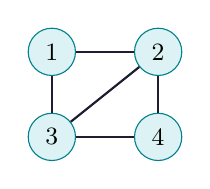
\begin{tikzpicture}[scale=0.9, every node/.style={circle, draw=myteal, fill=hdrteal, minimum size=0.6cm, font=\small}]
  \node (1) at (0,1.2) {1};
  \node (2) at (1.5,1.2) {2};
  \node (3) at (0,0) {3};
  \node (4) at (1.5,0) {4};
  
  \draw[line] (1) -- (2);
  \draw[line] (1) -- (3);
  \draw[line] (2) -- (4);
  \draw[line] (3) -- (4);
  \draw[line] (2) -- (3);
\end{tikzpicture}
\end{minipage}\hfill
\begin{minipage}{0.32\linewidth}
\centering
\textbf{Adjacency Matrix:}\par\noindent
{\renewcommand{\arraystretch}{1.2}%
\begin{tabular}{|c|c|c|c|c|}
\hline
& \textbf{1} & \textbf{2} & \textbf{3} & \textbf{4} \\
\hline
\textbf{1} & 0 & 1 & 1 & 0 \\
\hline
\textbf{2} & 1 & 0 & 1 & 1 \\
\hline
\textbf{3} & 1 & 1 & 0 & 1 \\
\hline
\textbf{4} & 0 & 1 & 1 & 0 \\
\hline
\end{tabular}}
\end{minipage}\hfill
\begin{minipage}{0.32\linewidth}
\centering
\textbf{Adjacency List:}\par\noindent
{\renewcommand{\arraystretch}{1.2}%
\begin{tabular}{|l|l|}
\hline
\textbf{Node} & \textbf{Neighbors} \\
\hline
1 & 2 $\rightarrow$ 3 \\
\hline
2 & 1 $\rightarrow$ 3 $\rightarrow$ 4 \\
\hline
3 & 1 $\rightarrow$ 2 $\rightarrow$ 4 \\
\hline
4 & 2 $\rightarrow$ 3 \\
\hline
\end{tabular}}
\end{minipage}
\end{tcolorbox}

\subsection{Bipartite Graphs in VLSI}
A graph $G = (V, E)$ is \textbf{bipartite} if its vertices can be partitioned into two disjoint sets $U$ and $W$ such that every edge $e \in E$ connects a vertex in $U$ to a vertex in $W$ (no edges exist between vertices of the same set). Bipartite graphs are used to represent:
\begin{itemize}[leftmargin=*, itemsep=2pt]
  \item Pin-to-net connectivity lists in floorplanning.
  \item Left-Edge algorithm horizontal/vertical routing constraints.
  \item Hardware binding/allocation problems.
\end{itemize}

\subsection{Tractability and Complexity Classes}
VLSI design problems involve thousands of components, making algorithm efficiency critical. We classify problems into complexity classes:
\begin{itemize}[leftmargin=*, itemsep=2pt]
  \item \textbf{Class P:} Problems solvable in polynomial time $O(n^k)$ by a deterministic Turing machine. Example: Shortest path routing.
  \item \textbf{Class NP:} Decision problems whose solutions are verifiable in polynomial time by a deterministic machine (or solvable in polynomial time by a non-deterministic Turing machine).
  \item \textbf{NP-Complete:} The hardest problems in Class NP. If a polynomial-time algorithm exists for any NP-complete problem, then $P = NP$. Example: Partitioning, Floorplanning, and Routing.
  \item \textbf{NP-Hard:} Problems at least as hard as any NP-complete problem, but not necessarily in NP (often optimization problems).
\end{itemize}

Since most physical design steps (partitioning, placement, routing) are NP-hard optimization problems, VLSI CAD tools must use \textbf{heuristic algorithms} (like simulated annealing, genetic algorithms) to find near-optimal solutions in reasonable computing time.

\subsection{Data Structures \& Algorithms in VLSI CAD}
VLSI design automation tools utilize classic computer science data structures and algorithms to model, analyze, and optimize physical circuits:

\par\vspace{6pt}\noindent
{\renewcommand{\arraystretch}{1.35}%
\begin{tabularx}{\linewidth}{|B{3.2cm}|Y|Y|}
\hline
\textbf{Concept} & \textbf{VLSI Application / Example} & \textbf{Core Role in Automation} \\
\hline
Graphs \& Hypergraphs & Netlists, routing grids, horizontal/vertical constraint graphs. & Models pin connectivity and track ordering. \\
\hline
Adjacency Matrix/List & Grid representation, component connection lists. & Back-end database for topological analysis. \\
\hline
Trees (Steiner / Slicing) & Global routing trees, slicing floorplan blocks, BDDs. & Optimizes wirelength, layout structures, and Boolean functions. \\
\hline
Priority Queues (Heaps) & Time-wheel event simulation, list scheduling priority queues. & Tracks next scheduled simulation events or operations. \\
\hline
Dijkstra / BFS / DFS & Maze routing (Lee's algorithm), reachability analysis. & Finds shortest routing paths around layout obstacles. \\
\hline
Graph Coloring & Register binding / allocation during HLS. & Assigns registers to non-overlapping variable lifetimes. \\
\hline
\end{tabularx}}

% ===============================================================================
\section{Combinatorial Optimization \& Heuristic Methods}
% ===============================================================================

\subsection{1. Simulated Annealing (SA)}
Simulated Annealing is a stochastic global optimization technique inspired by the process of physical annealing in metallurgy, where a metal is heated to a high temperature and cooled slowly to reach a low-energy, highly ordered crystalline state.

\begin{tcolorbox}[defbox, title={Simulated Annealing Core Principle}]
  To escape local minima, Simulated Annealing occasionally accepts worse moves (uphill steps) with a probability that decreases as the temperature decreases. This probability is governed by the Boltzmann distribution:
  \begin{equation}
    P(\text{accept}) = e^{-\frac{\Delta E}{T}}
  \end{equation}
  where $\Delta E = \text{Cost}(S_{\text{new}}) - \text{Cost}(S_{\text{current}})$ is the change in cost, and $T$ is the current temperature.
\end{tcolorbox}

\subsubsection{Algorithmic Flow}
\begin{enumerate}[leftmargin=*, itemsep=2pt]
  \item \textbf{Initialization:} Start with an initial configuration $S_0$ and a high initial temperature $T_0$.
  \item \textbf{Perturbation:} Make a small random change to the configuration to generate a neighbor state $S'$.
  \item \textbf{Cost Evaluation:} Compute $\Delta E = \text{Cost}(S') - \text{Cost}(S)$.
  \item \textbf{Acceptance Criteria:}
    \begin{itemize}[leftmargin=*, label=$\bullet$, itemsep=1pt]
      \item If $\Delta E < 0$ (improvement), accept the new state ($S \leftarrow S'$).
      \item If $\Delta E \ge 0$ (worse state), accept $S'$ only if a random number $r \in [0, 1)$ satisfies $r < e^{-\frac{\Delta E}{T}}$. Otherwise, reject it and keep $S$.
    \end{itemize}
  \item \textbf{Cooling:} Reduce the temperature using a cooling function (typically $T_{k+1} = \alpha T_k$, where $0.85 \le \alpha \le 0.98$).
  \item \textbf{Termination:} Repeat until $T$ reaches the stopping temperature $T_f$ or the system freezes.
\end{enumerate}

\begin{tcolorbox}[tikzbox, title={Simulated Annealing Flow Chart}]
\centering
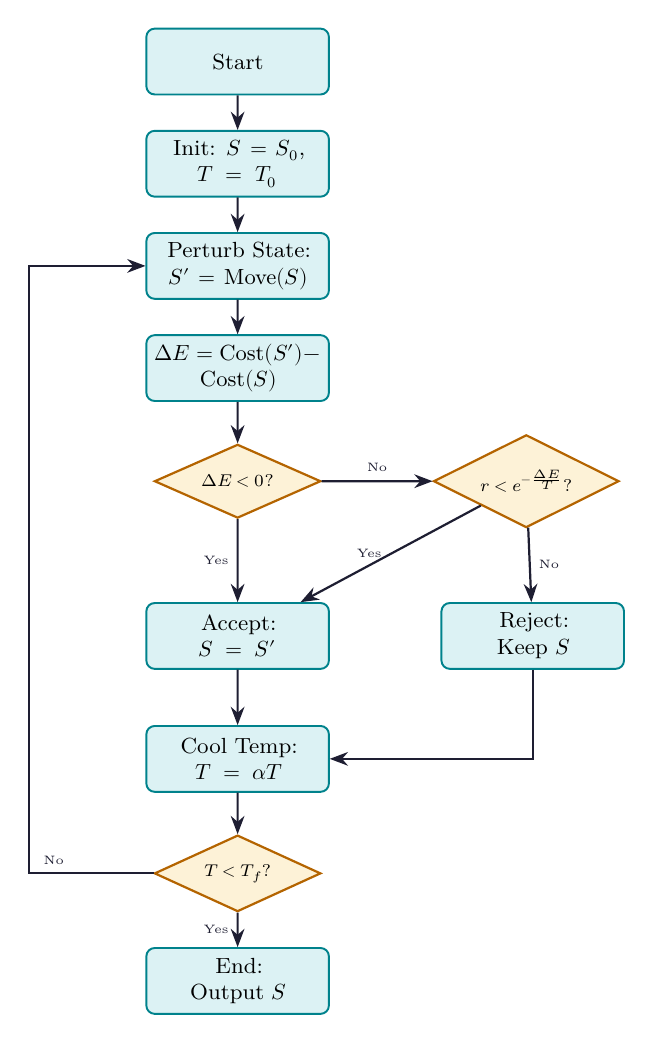
\begin{tikzpicture}[scale=0.88, transform shape, node distance=1.3cm]
  \tikzset{decision/.style={draw=myamber, fill=hdramber, diamond, aspect=2, minimum width=2.4cm, minimum height=1.0cm, align=center, font=\scriptsize, line width=0.8pt}}
  
  \node[block] (start) {Start};
  \node[block, below=0.5cm of start] (init) {Init: $S = S_0$,\\$T = T_0$};
  \node[block, below=0.5cm of init] (move) {Perturb State:\\$S' = \text{Move}(S)$};
  \node[block, below=0.5cm of move] (diff) {$\Delta E = \text{Cost}(S') - \text{Cost}(S)$};
  \node[decision, below=0.6cm of diff] (cond1) {$\Delta E < 0$?};
  
  \node[decision, right=1.6cm of cond1] (cond2) {$r < e^{-\frac{\Delta E}{T}}$?};
  \node[block, below=1.2cm of cond1] (accept) {Accept:\\$S = S'$};
  \node[block, right=1.6cm of accept] (reject) {Reject:\\Keep $S$};
  \node[block, below=0.8cm of accept] (cool) {Cool Temp:\\$T = \alpha T$};
  \node[decision, below=0.6cm of cool] (cond3) {$T < T_f$?};
  \node[block, below=0.5cm of cond3] (end) {End:\\Output $S$};
  
  % Connections
  \draw[arrow] (start) -- (init);
  \draw[arrow] (init) -- (move);
  \draw[arrow] (move) -- (diff);
  \draw[arrow] (diff) -- (cond1);
  \draw[arrow] (cond1) -- node[left, font=\tiny] {Yes} (accept);
  \draw[arrow] (cond1) -- node[above, font=\tiny] {No} (cond2);
  \draw[arrow] (cond2) -- node[left, font=\tiny] {Yes} (accept);
  \draw[arrow] (cond2) -- node[right, font=\tiny] {No} (reject);
  \draw[arrow] (accept) -- (cool);
  \draw[arrow] (reject) |- (cool);
  \draw[arrow] (cool) -- (cond3);
  \draw[arrow] (cond3) -- node[left, font=\tiny] {Yes} (end);
  
  % Loopback
  \draw[arrow] (cond3.west) -- node[above, pos=0.8, font=\tiny] {No} ++(-1.8,0) |- (move.west);
\end{tikzpicture}
\end{tcolorbox}

\subsection{2. Genetic Algorithms (GA)}
Genetic Algorithms are population-based heuristics inspired by natural selection and evolutionary biology.
\begin{itemize}[leftmargin=*, itemsep=2pt]
  \item \textbf{Representation:} Designs (e.g., placements) are encoded as strings of symbols called chromosomes.
  \item \textbf{Evaluation:} A fitness function determines the quality of each chromosome (e.g., inverse of total wirelength).
  \item \textbf{Crossover:} Pairs of chromosomes (parents) are combined with a probability $P_c$ to create offspring.
  \item \textbf{Mutation:} Random bits in the offspring chromosomes are inverted with a small probability $P_m$ to maintain genetic diversity and prevent premature convergence.
  \item \textbf{Selection:} Fitter individuals are selected to form the next generation.
\end{itemize}

\subsection{3. Integer Linear Programming (ILP)}
ILP is a mathematical optimization method where both the objective function and the constraints are linear equations, and the decision variables are restricted to integers.
\begin{itemize}[leftmargin=*, itemsep=2pt]
  \item Used for exact placement, routing track allocation, and resource scheduling.
  \item Yields the global optimum but suffers from high computational complexity (NP-complete), making it practical only for small design subproblems.
\end{itemize}

\newpage

% ═══════════════════════════════════════════════════════════════════════════════
% QUICK REVISION PAGE
% ═══════════════════════════════════════════════════════════════════════════════
\begin{center}
  {\large\bfseries\color{myred} Quick Revision — Module 1}\\[3pt]
  {\small\color{mydark} Introduction to VLSI Design Automation $|$ PE-EC802C}
\end{center}
\noindent{\color{myred}\rule{\linewidth}{1.2pt}}
\vspace{8pt}

\begin{tcolorbox}[formulabox, title={\textbf{Key Formulas and Metrics at a Glance}}]
\renewcommand{\arraystretch}{1.35}
\begin{tabularx}{\linewidth}{B{5.0cm} X}
  Boltzmann Probability & $P(\text{accept}) = e^{-\frac{\Delta E}{T}} \quad (\text{accepts uphill moves when } T \text{ is high})$ \\[4pt]
  Geometric Cooling Schedule & $T_{k+1} = \alpha T_k \quad (0.85 \le \alpha \le 0.98)$ \\[4pt]
  Degree Sum Theorem & $\sum_{v \in V} \text{deg}(v) = 2|E| \quad (\text{Handshaking Lemma})$
\end{tabularx}
\end{tcolorbox}

\vspace{6pt}

\begin{tcolorbox}[defbox, title={\textbf{One-Line Definitions}}]
\begin{itemize}[leftmargin=*, itemsep=3pt, topsep=0pt]
  \item \textbf{Y-Chart:} A representation of hardware design along Behavioral, Structural, and Physical axes.
  \item \textbf{Heuristic:} An approximate algorithm designed to solve NP-hard optimization problems in polynomial time.
  \item \textbf{Bipartite Graph:} A graph whose vertices are split into two disjoint sets, with edges only running between them.
  \item \textbf{Tractability:} The property of a problem indicating whether it can be solved within polynomial time.
  \item \textbf{Crossover:} The genetic algorithm operator that merges features of two parent chromosomes to create offspring.
  \item \textbf{Compaction:} The physical design phase that squeezes layouts to minimum area without violating design rules.
\end{itemize}
\end{tcolorbox}

\vspace{6pt}

\begin{tcolorbox}[exambox, title={\textbf{Frequently Asked / Viva Questions}}]
\begin{enumerate}[leftmargin=*, topsep=0pt, label=\textbf{Q\arabic*.}, itemsep=6pt]
  \item \Q{Why is physical design automation necessary in modern chip design?}
        Modern chips contain billions of transistors. Manual design is impossible due to complexity, human error, and time-to-market constraints. Automation ensures optimization, design rule compliance, and correct-by-construction layout generation within a few days.
        
  \item \Q{What are the typical cost components optimized during cell placement?}
        The placement phase optimizes: (1) Total wirelength (usually estimated using half-perimeter wirelength or HPWL), (2) Chip bounding box area, (3) Routing congestion, and (4) Critical path timing delays.
        
  \item \Q{Explain the metallurgical analogy used in Simulated Annealing.}
        In physical annealing, metal is heated to melt bonds (high energy, random atom states) and cooled very slowly. Atoms settle into a stable crystal lattice (minimum energy state). In Simulated Annealing, the configuration represents atom positions, cost represents system energy, and the control parameter $T$ acts as the temperature. High $T$ allows random moves, while slow cooling lets the algorithm settle into a global minimum cost state.
        
  \item \Q{What is the difference between NP-complete and NP-hard problems?}
        NP-complete problems belong to class NP (their solutions can be verified in polynomial time) and are at least as hard as any other problem in NP. NP-hard problems are not necessarily in NP (verification might not run in polynomial time), but any NP-complete problem can be reduced to them in polynomial time.
        
  \item \Q{Why can't we use exact methods like Integer Linear Programming (ILP) for whole-chip routing?}
        ILP is an NP-complete problem. The execution time of ILP solvers increases exponentially with the number of integer variables. Since modern chips contain millions of nets, solving a single global ILP formulation would take years. Hence, heuristics are used instead.
        
  \item \Q{How does the mutation parameter prevent premature convergence in Genetic Algorithms?}
        Premature convergence occurs when the population becomes uniform, trapped in a local minimum. Mutation randomly alters individual chromosome bits, reintroducing lost genetic traits and letting the algorithm explore untested search space regions.
        
  \item \Q{What is a hypergraph, and how is it used in circuit partitioning?}
        A hypergraph is a generalization of a graph where an edge (called a hyperedge) can connect any number of vertices. In VLSI, standard cells are vertices, and multi-terminal nets connecting three or more pins are represented as hyperedges.
        
  \item \Q{What role does the parameter $\alpha$ play in Simulated Annealing?}
        The parameter $\alpha$ is the cooling rate. If $\alpha$ is too small (e.g. 0.5), the temperature falls too rapidly, causing the system to freeze into a poor local minimum. If $\alpha$ is too close to 1 (e.g. 0.999), the cooling is extremely slow, and the algorithm takes too long to run. Standard values are between $0.85$ and $0.98$.
        
  \item \Q{What is the difference between top-down and bottom-up design methodologies?}
        Top-down starts with a high-level specification and refines it down to RTL, gate-level, and finally transistor layout. Bottom-up starts by designing individual custom circuits, standard cells, or sub-blocks, and then joins them to build the complete system.
        
  \item \Q{Why does routing require two separate steps: Global Routing and Detailed Routing?}
        Routing is highly complex. Solving it in one step is computationally impossible. Global routing simplifies the problem by dividing the chip into a coarse grid and routing nets through grid regions without assigning specific tracks. Detailed routing then focuses on each grid region separately to assign nets to precise metal tracks and layers.
\end{enumerate}
\end{tcolorbox}

\vspace{6pt}

\begin{tcolorbox}[tikzbox, title={\textbf{Comparison Snapshot}}]
\textbf{Structural vs. Behavioral Domain:}\par\vspace{6pt}\noindent
{\renewcommand{\arraystretch}{1.35}%
\begin{tabularx}{\linewidth}{|B{3.2cm}|Y|Y|}
\hline
\textbf{Feature} & \textbf{Behavioral Domain} & \textbf{Structural Domain} \\
\hline
Description & Focuses on algorithmic functionality and logic transitions. & Focuses on hardware components and connectivity netlists. \\
\hline
Example & Transfer functions, state equations, Boolean expressions. & Logic gates, flip-flops, ALUs, multiplexers. \\
\hline
Representation & VHDL/Verilog process blocks, C/C++ behavior models. & Structural netlists, schematic diagrams. \\
\hline
\end{tabularx}}

\vspace{12pt}
\textbf{Class P vs. Class NP Problems:}\par\vspace{6pt}\noindent
{\renewcommand{\arraystretch}{1.35}%
\begin{tabularx}{\linewidth}{|B{3.2cm}|Y|Y|}
\hline
\textbf{Feature} & \textbf{Class P} & \textbf{Class NP} \\
\hline
Solvability & Solvable in polynomial time by a deterministic machine. & Solvable in polynomial time by a non-deterministic machine. \\
\hline
Verification & Can be solved and verified in polynomial time. & Solutions can be verified in polynomial time. \\
\hline
VLSI Example & Shortest-path routing (Dijkstra's). & Cell placement, partition minimization, floorplan sizing. \\
\hline
\end{tabularx}}
\end{tcolorbox}

\end{document}
